
\begin{table}[htbp]
  \caption{汇款账户(APS 注册成功后会自动生成该表格内容)}
  \label{tb:bank-account}
  \centering
  \begin{tabular}{ll}
    \toprule
    收款人名称 & 德国驻华使馆文化处留德人员审核部 \\
    帐号 & 332 456 013 427 \\
    收款银行名称 & 中国银行北京亮马河大厦支行 \\
    \bottomrule
  \end{tabular}
\end{table}

\begin{center}
\begin{tabular}{ll}
  \toprule
  目的 & 境外银行\textbf{开户} \\ \midrule
  需要证明 & \textbf{资金来源证明(存款证明),\color{blue}中英文},同一张纸上即可 \\ \midrule
  方式 & 在任意一家可办理\textbf{\color{blue}境外汇款业务}的银行,\\
  & (中国银行、建行、工商银行、农行均可) \\
  & 冻结约 9000 \textbf{\color{blue}欧元}(不必过多), \\
  & 并要求银行开具\textbf{资金来源证明}或\textbf{存款证明}。该证明上时间只需持续一天。 \\
  & 如 2018 年 12 月 20 日至 2018 年 12 月 21 日。 \\
  冻结时间 & 约 2 周。(这段时间学生会去申请开户) \\ \midrule
  邮寄 & 将该证明\textbf{原件}邮寄过来。 \\ \midrule
  汇款 & {\color{blue}时间}: 学生办理开户后,通知汇款时间。 \\
  & {\color{blue}金额}: 与开户时填写数目一致(以\textbf{\color{blue}欧元}汇出)。 \\
  & {\color{blue}汇款人}: \textbf{资金证明的账户\color{blue}持有人}! \\
  & {\color{blue}汇款地址}: 见下页表格 \\
  & \textbf{一次性汇出。金额不多不少。} \\
  & 填写汇款人住址时还需写清所在\textbf{城市}。 \\
  & 国内外费用承担建议选择:共同 SHA。 \\
  & 如汇款行要求填写收款人地址,可使用收款人开户银行的地址信息。 \\ \midrule
  \textbf{汇款后} & 在汇出行完成国家外汇管理局要求的\textbf{跨境支出申报}。 \\  
  \bottomrule
\end{tabular}
\end{center}

% \newpage

\begin{table}
\caption{汇款地址信息}
\label{tb:address}
\begin{center}
\begin{tabular}{l}
\toprule
收款人开户银行名称及地址(57): Deutsche Bank AG, Frankfurt H.O. \\
\multicolumn{1}{c}{Taunusanlage 12, 60325 Frankfurt, Germany
 (SWIFT: DEUTDEFFXXX)} \\
收款人名称(59): Deutsche Bank (China) Student BJ \\
收款人账号(59): IBAN: DE64 5007 0010 0951 2724 01 \\
汇款附言(70): 开户人姓名拼音 (大写): \underline{\hspace*{3cm}} 个人编号 (REFERENCE NUMBER):\\
 $\rule{3cm}{0.15mm}$(共 9 位组成) \\ \bottomrule
\end{tabular}
\end{center}
\end{table}

\newpage

\begin{table}[htbp]
\caption{2018 年 12 月 19 日德意志银行开户体验(及后续同学完善)}
\label{tb:opening-Dec-19}
\centering
\begin{tabular}{l}
\toprule
出发地点:玉泉路 \\
出发时间: 9: 02 \\
到达地点:朝阳区建国路 81 号华贸中心 27 层 \\
到达时间: 9: 55 \\
取号等待 \\
办理开户 \\ \bottomrule
\end{tabular}
\end{table}
\noindent
备注:
\begin{description}
\item[一年/半年期] LHB 同学已得到德国使馆邮件(图 \ref{fig:email})回复,一年期限制提款和半年期限制题款均可。注意,二者的扣款情况,除开户手续费 (850 / 1200 元人民币) 外,还有可能存在按比例收取的转账手续费。如需了解,请提前向本地银行确认。此外,无论是一年期还是半年期,均可以自由支取冻结金额以外的存款。
\begin{figure}[htbp]
  \centering
  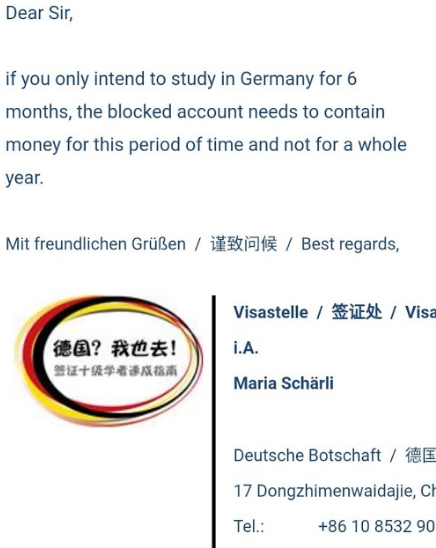
\includegraphics[height=.5\textheight]{email-from-Visa}
  \caption{德国使馆回信}
  \label{fig:email}
\end{figure}
\item[行程] 地铁一号线大望路站,刷卡(码)出站后,顺着 \textbf{\color{blue}A (东北)口}出站方向,前行约十米,沿着\textbf{\color{blue}“华贸中心”通道}前行。进入“华贸中心”(B1,负一层)后,按指示路牌 \textbf{\color{blue}“华贸写字楼”} 方向前行至一上行扶梯处。出扶梯左手入口即有``Deutsche Bank'' 标志。有服务人员在柜台等候。按指示在机器上选 27 层德意志银行,得到二维码。刷码进入写字中心。乘梯至 27 层,左手即为德意志银行。
\item[表格]
\begin{itemize}
  \item 请务必下载 \href{https://china.db.com/china/docs/1.opening\_a\_bank\_account\_for\_foreign\_students\_over18years.pdf}{\textbf{\color{blue}官方最新版表格}}. 填写完整后打印 ``Guidance notes'' 后的所有页(文档当前版本:
  007 91995 28 DBEN 164 WWW ERO BV VJ \textbf{\color{blue}181024} 的\textbf{\color{blue}第 9 -- 19 页}),包括 ``Schufa'' 1 页, ``Entgeltinformation'' 3 页和 ``Depositor Information Sheet'' 1 页。 
  \item 请确保自动生成了 ``\textbf{\color{blue}First name/s}'', ``\textbf{\color{blue}Surname}'' 两栏
  \item 身份证、护照页复印件\textbf{避免过黑}。在空白处写上个人 “姓名” + “拼音”(此前已经有人建议姓名全部大写。我全部大写了)
  \item 按照工作人员的意思,邮寄可能比自取\textbf{\color{blue}晚“一到两天”}。我选了邮寄。邮寄方式为 EMS. 周一向德意志银行学生账户成功汇款,当周五拿到德意志银行的 EMS 开户证明。
  \item 银行张贴的开户示例与官网示例稍有不同---主要是“城市”全部写成“\textbf{\color{blue}省份+城市}”(或城市+省份。可由逗号或空格分隔。下同)。我拍了前两张,将发群里。
  \begin{itemize}
    \item ``Place of birth'' 省份 + 城市
    \item ``Regestered address'' 中 ``Town/City'' 省份 + 城市。我填了 ``BeijingShijingshan''. 没有空格,因为格数不够。
    \item ``My relationship with this person is as follows (e.g. father/son)'' 我填写了 ``Mother\textbf{\color{blue}/Son}''. 注意,后面的 ``/Son(/Daughter)'' \textbf{\color{blue}不可省}。
  \end{itemize}
\item JHX: 材料不要订起来
\item 据说华贸大厦马路对面有家打印店,可搜索到。打印费较贵, 0.5 元/张(ZZY:“那边打印店 2 元一张)。但我高德地图搜不到。仅需打印修改过的页面。{\color{blue}无需打印自己保留的那一份}。我是托旁边人一起打印的,打印店具体位置等不清楚。而且请注意{\color{blue}打印不清晰的,应要求重新打印}。我有几页打印太不清晰。幸好那几页所有人都相同,台湾的一位朋友把他剩余的那几页给了我。
\item 由于去中国银行、工商银行(均在华贸中心一楼。工商银行需转角出门再进。可询问服务台)\textbf{均需\color{blue}当前银行卡},暂不接受现金汇款;而我没有这两个银行的卡,于是我回到玉泉路建行汇出开户手续费。%据 ZJR 表示,德意志银行\textbf{\color{blue}不会通知}是否收到该笔汇款。我托ZZY明天问问德意志银行。
\\
% 这件事情最好有个彻底的处理方式。比如,要求银行受到汇款后发出通知。
ZZY:“关于汇款问题,假如你没汇款是会有电话通知。没问题就不会联系。”
\item 银行业务人员要求拍照保存自己填写的快递单。利用快递单,可以查看相应材料的运送进程。
\item 银行仅两个柜台。我当天仅一位业务人员。
\item 我全程感觉到的都是{\color{blue}和善}。业务人员也很耐心。本来办公时间只到 11:30, 但她允许我们最迟 12:00 递交材料。
\end{itemize}
\item[转账] 我利用建行网银向上述指定银行转账 8900 欧元。周一转出,当周五受到德银的“个人帐号通知函”(名称由申请开户时拿到的“个人编号通知单”推知)邮件。虽然过程中有以下小问题(及处理方式),但从结果来看,没有受到影响。
\begin{itemize}
  \item 建行网银转账时,输入对方账户名时,不能包含 ``Bank''. 我改为 "BK".
  \item 按开户表上填写的 8900 欧元,实际转出 8900 欧元。“个人帐号通知函”上显示,实际到帐 8870 欧元(应该是中转过程中扣除了 30 欧元)。
\end{itemize} 
\item[解冻] ( ZJR )回国前可以用\textbf{机票和学校的注销证明}去德意志银行解冻。
\end{description}